\documentclass[letterpaper,journal]{IEEEtran}
\usepackage{amsmath,amssymb,amsfonts}
\usepackage{booktabs}
\usepackage{graphicx}
\usepackage{cite}
\usepackage{url}
\usepackage[hidelinks]{hyperref}
\usepackage{xcolor}

\newcommand{\Tr}{\operatorname{Tr}}
\newcommand{\rank}{\operatorname{rank}}
\newcommand{\E}{\mathbb{E}}
\newcommand{\R}{\mathbb{R}}
\newcommand{\C}{\mathbb{C}}
\newcommand{\AOC}{\textsc{AOC}}

\begin{document}

\title{Additive Observable Contrast: Maximum-Difference Witnesses for Streaming Physical States}

\author{Rongzhou (Lachlan) Chen%
\thanks{Working paper. Code, fixed-seed records, and generated figures are
available in the accompanying public repository. This manuscript does not
claim a hardware implementation or a privacy guarantee.}}

\maketitle

\begin{abstract}
Principal components maximize variance, although the direction of largest
variance need not distinguish conditions. We formulate the original
maximum-class-difference motivation of Eigen-Component Analysis as
\emph{additive observable contrast} (\AOC). Each sample is encoded as a
positive trace-one operator; per-condition sums and masses are exactly
mergeable; and the bounded effect with the largest expectation change is the
positive spectral projector of the state difference. The resulting scalar is
trace distance, rank budgets have an analytic Ky Fan solution, and the
multiclass extension is the minimum-error positive-operator-valued-measurement
semidefinite program. A predictable online witness can be coupled to a betting
martingale when the reference state is known. Numerical audits match batch,
merged, kernel, and semidefinite formulations to at most
$6.7\times10^{-9}$. Matched physical tests expose the intended regime rather
than universal dominance: under exact sign symmetry, a linear Ising
classifier remains at $50\%$ while \AOC obtains $99.98\%$ and recovers the
magnetization mode; a rank-one structural witness obtains $0.977$ ROC AUC and
$0.993$ overlap with the analytical damage mode; and an optical analyzer
raises state-discrimination success from $50\%$ to $95\%$, reproduced by
finite-shot Qiskit Aer simulation. The method is therefore best viewed as a
mergeable, interpretable measurement-design primitive for state
discrimination, change detection, and mode localization, not as a universal
classifier.
\end{abstract}

\begin{IEEEkeywords}
change detection, density operators, interpretable learning, online
algorithms, quantum-inspired computing, state discrimination
\end{IEEEkeywords}

\section{Introduction}

\IEEEPARstart{V}{ariance} is valuable when the dominant fluctuation is also
the phenomenon of interest. It is misleading when a nuisance direction has
large variance, or when two conditions have the same mean and differ only in
power or coherence. The original Eigen-Component Analysis (ECA) work sought
features with large class difference rather than large pooled
variance~\cite{chen2025eca}. The question left open is what ``difference''
means, which constraints make it operational, and how the object should be
updated as observations arrive one at a time.

We answer these questions using positive operators. A normalized outer
product is simultaneously a second-order feature state, a kernel mean
embedding, an optical coherency state, and---when the data are quantum---a
density operator. A bounded quadratic readout is an \emph{effect}
$0\preceq E\preceq I$. The optimal difference is then not an analogy to
quantum theory; it is the binary state-discrimination problem solved by
Helstrom~\cite{helstrom1976,holevo2011}. This identification prevents an
incorrect novelty claim while supplying a precise foundation.

The contribution is a synthesis oriented toward streaming physical data:

\begin{enumerate}
\item We express maximum-difference feature learning as the positive part of
an additive state contrast, including exact rank-constrained and multiclass
forms.
\item We expose exact batch--online--merge equivalence and distinguish a valid
predictable sequential witness from a same-sample adaptive score.
\item We validate algebra, mode recovery, finite-shot measurement, and false
alarms from stored raw records, with explicit claim boundaries.
\end{enumerate}

This positioning addresses a practical distinction from covariance
generalized eigenmethods such as common spatial patterns (CSP)~\cite{parra2003}:
CSP optimizes a variance ratio under a reference metric, whereas \AOC\
optimizes an absolute bounded expectation gap after trace normalization.

\section{Positive-State Formulation}

\subsection{Additive encoding}

For a nonzero feature vector $\phi(x)\in\C^d$, define
\begin{equation}
 R(x)=\frac{\phi(x)\phi(x)^\dagger}{\|\phi(x)\|_2^2},
 \quad R(x)\succeq0,\quad \Tr R(x)=1.                 \label{eq:state}
\end{equation}
Condition $c$ is represented by
\begin{equation}
 S_c=\sum_i w_iR(x_i),\quad m_c=\sum_iw_i,\quad
 \rho_c=S_c/m_c.                                    \label{eq:additive}
\end{equation}
The statistic $(S_c,m_c)$ is exactly additive. It is constant in the number
of samples, but not private: outer-product sums can leak information, and
privacy requires a separate threat model and mechanism.

\subsection{Binary optimal effect}

Let $\Delta=\rho_1-\rho_0$ and let
$\Delta=\Delta_+-\Delta_-$ be its Jordan decomposition.

\textbf{Theorem 1 (maximum bounded contrast).}
For Hermitian $\Delta$,
\begin{equation}
\max_{0\preceq E\preceq I}\Tr(E\Delta)=\Tr(\Delta_+),\qquad
E^\star=\mathbf 1_{\Delta>0}.                       \label{eq:jordan}
\end{equation}

\begin{IEEEproof}
Because $0\preceq E\preceq I$,
$\Tr(E\Delta_+)\leq\Tr\Delta_+$ and
$-\Tr(E\Delta_-)\leq0$. Equality is obtained by the support projector of
$\Delta_+$, which is orthogonal to the support of $\Delta_-$.
\end{IEEEproof}

For trace-one inputs, $\Tr\Delta=0$ and therefore
\begin{equation}
\Tr\Delta_+=\tfrac12\|\Delta\|_1.                   \label{eq:trace}
\end{equation}
With equal priors this gives
$P_{\rm succ}^\star=1/2+\|\Delta\|_1/4$, the Helstrom
success probability~\cite{helstrom1976}. Quantum Chernoff theory addresses
the distinct many-copy error exponent~\cite{audenaert2007}.

\textbf{Corollary 1 (rank budget).}
If $\lambda_1\geq\cdots\geq\lambda_d$ are the eigenvalues of $\Delta$, then
\begin{equation}
\max_{\substack{0\preceq E\preceq I\\\rank(E)\leq r}}\Tr(E\Delta)
=\sum_{j=1}^r\max(\lambda_j,0).                     \label{eq:kyfan}
\end{equation}
The effect projects onto the retained positive eigenvectors. This is a
measurement-capacity constraint, not only a statistical penalty.

\subsection{Multiclass observations}

Independent one-versus-rest effects need not sum to a realizable measurement.
For $K$ class states and priors $\pi_c$, the coherent extension is
\begin{equation}
\begin{aligned}
\max_{\{E_c\}}\quad&
\sum_{c=1}^K\pi_c\Tr(E_c\rho_c),\\
\text{s.t.}\quad&E_c\succeq0,\qquad\sum_cE_c=I.     \label{eq:povm}
\end{aligned}
\end{equation}
This is the established minimum-error state-discrimination SDP~\cite{holevo2011}.
Its no-information baseline is $\max_c\pi_c$. Our implementation returns
primal feasibility diagnostics; tests obtain unit success on orthogonal
states, the prior baseline on identical states, and the Helstrom value for
$K=2$.

\subsection{Kernel interpretation}

For normalized feature rows, the projective kernel
\begin{equation}
k(x,z)=|\langle\phi(x),\phi(z)\rangle|^2
\end{equation}
has mean embedding $\rho$. Consequently,
\begin{equation}
\operatorname{MMD}_k^2(P,Q)=\|\rho_P-\rho_Q\|_F^2.  \label{eq:mmd}
\end{equation}
MMD~\cite{gretton2012} and \AOC\ use the same contrast operator but different
norms: MMD uses Hilbert--Schmidt magnitude, while \AOC\ uses trace magnitude
and produces a bounded witness. Neither norm guarantees universally better
finite-sample power.

\section{Streaming and Sequential Detection}

\subsection{Exact state operations}

An arrival performs $(S,m)\leftarrow(S+wR,w+m)$. Disjoint summaries merge by
addition. A retained observation can be removed, a fixed window can add and
subtract, and forgetting applies $(S,m)\leftarrow(\gamma S,\gamma m)$.
Associativity implies that centralized batch, arbitrary partitions, and
arbitrary merge trees return the same empirical state up to floating-point
roundoff. Communication of a dense Hermitian state costs $O(d^2)$ numbers per
merge, independent of sample count; diagonal, sparse, or low-rank structure
can reduce this cost.

\subsection{Predictable learned witness}

Same-sample optimization invalidates ordinary null calibration. Let $E_t$ be
measurable with respect to observations before time $t$, and suppose the
reference state $\rho_0$ is known. The score
\begin{equation}
z_t=\Tr[E_t(R_t-\rho_0)]\in[-1,1]                  \label{eq:score}
\end{equation}
has conditional mean zero under an independent stationary null. For
$0<\lambda<1$,
\begin{equation}
M_t(\lambda)=\prod_{i=1}^t(1+\lambda z_i)           \label{eq:martingale}
\end{equation}
is a nonnegative martingale. Mixtures over $\lambda$ and candidate start times
remain e-processes, yielding anytime evidence under their stated
assumptions~\cite{howard2021}. A plug-in reference estimate is diagnostic
unless its uncertainty is incorporated. Recent work already develops
universal quantum-observable change detection with classical shadows and
e-detectors~\cite{zecchin2026,huang2020}; therefore generic online quantum
change detection is not claimed as novel here.

\subsection{Complexity and stability}

Dense accumulation is $O(d^2)$ per state and a complete eigendecomposition is
$O(d^3)$. A rank-$r$ Lanczos update can use matrix--vector products without a
full decomposition. Witness orientation is stable only when the positive
spectral subspace has an eigengap; Davis--Kahan perturbation theory bounds its
rotation by estimation error divided by that gap~\cite{daviskahan1970}.
A small gap should therefore be reported as an identifiability warning even
when the scalar trace distance is stable.

\section{Reproducible Physical Tests}

\subsection{Protocols}

All scripts use fixed seeds, write raw CSV files, save software and Git
metadata, and hash outputs. The algebra audit samples random density
operators, random arrival orders, and random merge trees. The sequential audit
uses a known reference, previsible rank-one witnesses, and an alarm threshold
$1/\alpha$ with $\alpha=0.01$.

The Ising test uses $12\times12$ Wolff samples at $T=1.6$ and $3.5$. Every
configuration is paired with its global negative, making the empirical mean
exactly zero in both classes. The structural test is a 12-mass chain under
zero-mean thermal excitation; one spring loses stiffness. The optical test
uses diagonal/antidiagonal polarization states with visibility $0.9$ and
$16\,384$ shots per state in Qiskit Aer~\cite{qiskit2024}. These are controlled
physical models, not field deployments.

\begin{figure}[t]
\centering
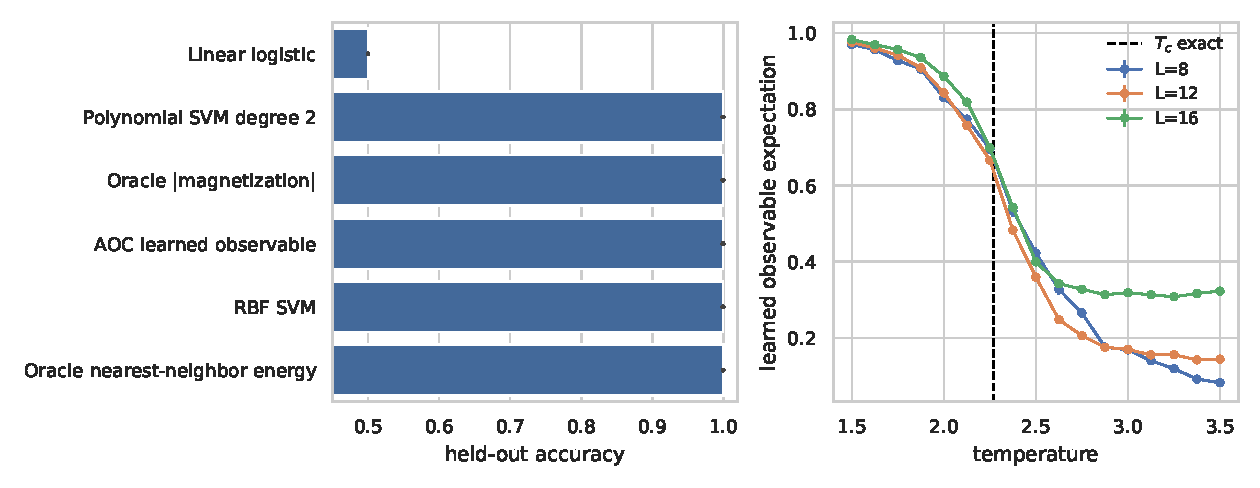
\includegraphics[width=\columnwidth]{../../experiments/run2/results/ising/ising_order.pdf}
\caption{Left: matched Ising classification. Right: the learned observable
tracks the finite-lattice order response. Linear failure is forced by exact
$Z_2$ pairing; nonlinear baselines correctly solve the task.}
\label{fig:ising}
\end{figure}

\begin{figure}[t]
\centering
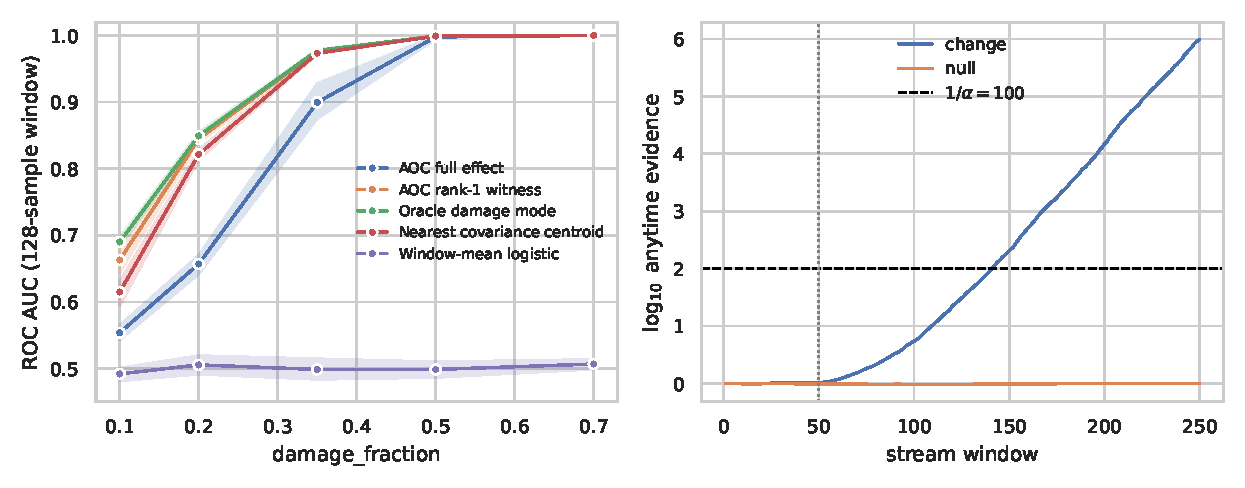
\includegraphics[width=\columnwidth]{../../experiments/run2/results/structural/structural_monitoring.pdf}
\caption{Structural damage under zero-mean excitation. A rank-one capacity
constraint approaches the planted mode and improves over the unrestricted
positive subspace.}
\label{fig:structure}
\end{figure}

\begin{table}[t]
\caption{Selected Held-Out Results}
\label{tab:results}
\centering
\small
\begin{tabular}{lcc}
\toprule
Experiment/method & Metric & Mean\\
\midrule
Ising linear logistic & accuracy & 0.5000\\
Ising \AOC & accuracy & 0.9998\\
Ising RBF SVM & accuracy & 0.9998\\
Structure mean logistic & ROC AUC & 0.4985\\
Structure rank-one \AOC & ROC AUC & 0.9768\\
Structure oracle mode & ROC AUC & 0.9774\\
Optics fixed H/V & success & 0.5000\\
Optics Helstrom/Aer & success & 0.9500\\
\bottomrule
\end{tabular}
\end{table}

\subsection{Results and interpretation}

The algebra audit finds maximum batch/additive density error
$3.60\times10^{-16}$, merge-mass error $9.95\times10^{-14}$, analytic/SDP
Jordan gap error $6.67\times10^{-9}$, trace identity error
$2.22\times10^{-16}$, and kernel/operator error $2.78\times10^{-16}$.

Figure~\ref{fig:ising} and Table~\ref{tab:results} show the intended
mean-blind regime. \AOC\ reaches $0.9998\pm0.0007$ accuracy and its leading
vector has mean squared overlap $0.9991$ with the uniform magnetization mode.
The comparison is not universal dominance: the RBF SVM ties \AOC, the
degree-two SVM reaches $0.9996$, and the physical energy oracle is perfect.
The contribution is analytic recovery of an interpretable order mode from a
mergeable state.

At $35\%$ spring damage and 128-sample windows, Fig.~\ref{fig:structure} gives
ROC AUC $0.9768$ for rank-one \AOC, $0.9733$ for nearest covariance centroid,
$0.9774$ for the oracle damage mode, and $0.4985$ for window-mean logistic.
The learned/analytical damage-mode overlap is $0.9935$ on average. Full
positive-subspace \AOC\ is worse ($0.8996$ AUC), demonstrating that maximizing
population mean gap need not minimize finite-window decision error when extra
modes add variance.

\begin{figure}[t]
\centering
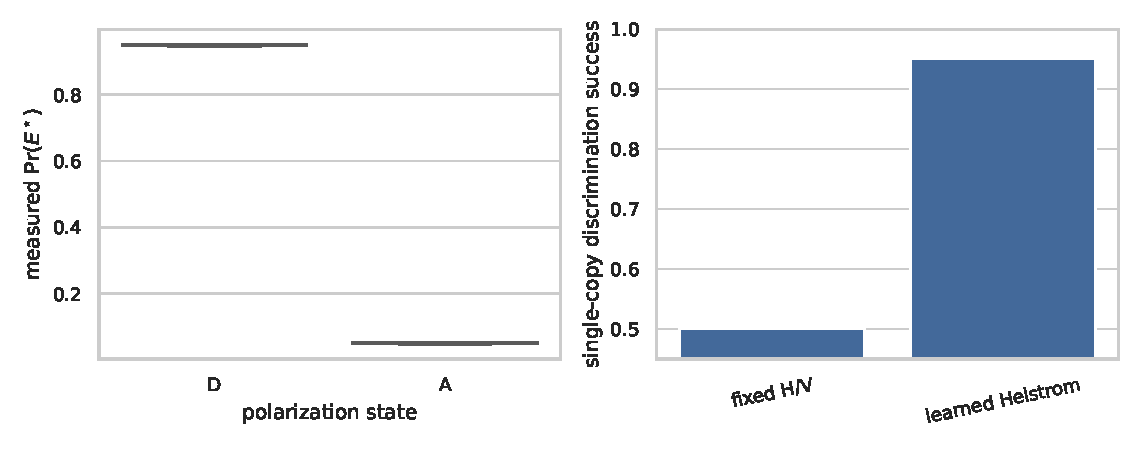
\includegraphics[width=\columnwidth]{../../experiments/run2/results/optics/optical_quantum.pdf}
\caption{Optical state discrimination. The optimal Bloch-axis analyzer
replaces a deliberately blind horizontal/vertical analyzer; Aer sampling
matches the analytic probability.}
\label{fig:optics}
\end{figure}

In Fig.~\ref{fig:optics}, the learned effect has Bloch vector $(1,0,0)$.
The trace distance is $0.9$, giving theoretical success $0.95$ rather than
$0.5$ for fixed horizontal/vertical readout. Across 20 seeds, Aer gives
$0.950009\pm0.000996$ with maximum probability error $0.003125$, one qubit,
and transpiled depth two. This is a measurement-basis result, not a quantum
speedup claim.

In the general sequential audit, 2 of 500 stationary streams alarm
(empirical rate $0.004$; exact binomial 95\% upper bound $0.0144$), while all
200 changed streams alarm with median delay 30. In the more conservative
structural stream, 0 of 120 nulls and all 120 changes alarm, with median delay
89 after a $70\%$ damage change. These finite simulations audit the
implementation but do not extend the theorem beyond a known independent
reference.

\section{Scope, Limitations, and Applications}

The outer-product encoding loses global sign and phase. This is beneficial in
the Ising, power, and coherency tasks but makes phase-coded or homometric
signals indistinguishable. Higher tensor powers or phase-retaining feature
maps are needed. Dense storage scales as $d^2$, eigensolvers can dominate,
and empirical states can be poorly conditioned when $d$ is large. The
multiclass SDP scales less favorably than the binary eigendecomposition.

\AOC\ is promising where the observable itself has physical meaning:
polarization/coherence analyzers~\cite{wolf2007}, ambient-vibration covariance
changes~\cite{wang2010damage}, order parameters in phase
discovery~\cite{carrasquilla2017}, force/torque contact modes, and quantum
device drift. Each domain requires its own nuisance model, instrument
constraints, and real-data validation.

The decisive condition is not ``machine learning'' but a match between the
state representation and the phenomenon: if the change lies in a low-rank
operator moment while means cancel, a bounded quadratic witness can be both
sample-efficient and interpretable. If the difference lies outside that
moment, the method is blind by construction.

\section{Conclusion}

\AOC\ turns the qualitative goal of maximizing class difference into an exact
measurement-design problem. The binary solution is a positive spectral
projector, rank constraints select positive Ky Fan modes, multiclass
classification is a POVM SDP, and all inputs can be accumulated and merged
exactly. The experiments establish strong performance only in matched
mean-blind physical regimes and expose ties and failures. The next step is to
restrict observables to known symmetries or instrument algebras and resolve
which physical sector carries the distinguishability.

\bibliographystyle{unsrt}
\bibliography{references}

\end{document}
